% \documentclass[a4paper,twocolumn]{jsarticle}
\documentclass[a4j,twocolumn]{ujarticle} % 'jsarticle' が使えない場合はこちらを利用

% 上記 documentclass のオプションは自由に追加してもよい.

%%%%%%%%%%%%%%%%%%%%%%%%%%%%%%%%%%%%%%%%%%%%%%%%%%%%%%%%%%%%%%%%%%%%%%%%%%%%%%
%%% ページ設定 (この項目は論文著者は編集しないこと.)

% 芸術科学会学術会議用スタイルパッケージ
\usepackage{artsci-conf-j}

% 開始ページ数設定
\setcounter{page}{1}

% ヘッダスタイル
\markright{\footnotesize{
\textbf{NICOGRAPH 20xx, pp. aaa -- bbb}
}}
\pagestyle{myheadings}

%%%%%%%%%%%%%%%%%%%%%%%%%%%%%%%%%%%%%%%%%%%%%%%%%%%%%%%%%%%%%%%%%%%%%%%%%%%%%%
%%% パッケージ一覧 (必要なパッケージを任意に追加してよい)

\usepackage{amsmath, amssymb}	% AMS-LaTeX
\usepackage[dvipdfmx]{graphicx}	% 「graphics」パッケージに変更してもよい.
\usepackage{float}		% 図表が記述位置から飛ばないためのパッケージ
\usepackage{url}		% URL 表記用パッケージ

%%%%%%%%%%%%%%%%%%%%%%%%%%%%%%%%%%%%%%%%%%%%%%%%%%%%%%%%%%%%%%%%%%%%%%%%%%%%%%
%%% 画像ファイルの include path
\graphicspath{{fig/}} %% グラフィック用


%%%%%%%%%%%%%%%%%%%%%%%%%%%%%%%%%%%%%%%%%%%%%%%%%%%%%%%%%%%%%%%%%%%%%%%%%%%%%%
%%% マクロ一覧 (必要なマクロをこの部分に記述)

\newcommand{\bA}{\mathbf{A}}
\newcommand{\bB}{\mathbf{B}}


%%%%%%%%%%%%%%%%%%%%%%%%%%%%%%%%%%%%%%%%%%%%%%%%%%%%%%%%%%%%%%%%%%%%%%%%%%%%%%
%%% タイトル,著者,所属,概要

% 日本語タイトル
\jtitle{
色名に用いられる漢字による〜〜可視化手法の提案と考察
}

% 英語タイトル
\etitle{
Using kanji for color name ~~ visualization
}

% 日本語著者
% 所属参照は好みに応じて \dagger などを用いてもよい.
\jauthor{
遠藤勝也\(^{1)}\){\small (非会員)}
% ~~~ % 氏名の間隔はチルダ記号や hspace 等で適宜調節のこと.
% 科学次郎\(^{2)}\){\small (正会員)}
}

% 英語著者
\eauthor{
Katsuya Endoh\(^{1)}\)
% ~~~
% Jiro Kagaku\(^{2)}\)
}

% 日本語所属
\jaffiliation{
1) 株式会社スタジオ・アルカナ
% ~~~
% 2) 芸術科学大学芸術科学部
}

% 英語所属
\eaffiliation{
1) Studio Arcana co.,Ltd.\\
% 2) Department of Art and Science, The University for Art and Science
}

% 連絡先電子メールアドレス(省略可)
% (スパム対策は著者自身の判断によって措置すること.
% このサンプルでは「@」を2バイト文字にすることで対応してある.)
\email{
endkty0509@gmail.com
}

% 日本語概要
\jabstract{
深緋(こきあけ)は,RGB値では(201, 23, 30)のように表現できるが.
これらの数値から,濃い赤と想像できるが,
色を数値で扱う習慣がなければ,想像することは難しいと考えられる.
しかし,深緋という色名に用いられている漢字に注目すると,
「深」と「緋」の二つの漢字が使われている.
表意文字である漢字は,
「深」という漢字からは暗さや濃さ,
「緋」という漢字は赤に近い色のように,
意味を想起させられる.
そこで本研究では,色名に用いられている漢字に注目し分析し,
漢字を色空間内のベクトルとして表現することで,
漢字が色イメージに与えるベクトルを推測し,その結果を考察する.
}

%%%%%%%%%%%%%%%%%%%%%%%%%%%%%%%%%%%%%%%%%%%%%%%%%%%%%%%%%%%%%%%%%%%%%%%%%%%%%%
% ここより論文本体

\begin{document}
\maketitle
\thispagestyle{myheadings}

\section{はじめに}

深緋(こきあけ)は,RGB値では(201, 23, 30)のように表現できるが.
これらの数値から,濃い赤と想像できるが,
色を数値で扱う習慣がなければ,想像することは難しいと考えられる.
しかし,深緋という色名に用いられている漢字に注目すると,
「深」と「緋」の二つの漢字が使われている.
表意文字である漢字は,
「深」という漢字からは暗さや濃さ,
「緋」という漢字は赤に近い色のように,
意味を想起させられる.
そこで本研究では,色名に用いられている漢字に注目し分析し,
漢字を色空間内のベクトルとして表現することで,
漢字が色イメージに与えるベクトルを推測し,その結果を考察する.

\section{先行研究}

\subsection{ページ設定およびページ数}

論文本体のページ設定は A4 とする.このページ設定で不都合なコンテンツがある場合は,
静止画であっても論文本体に含めずに添付ファイルで提出していただきたい.

論文本体のページ数は,各会議で規定される通りとする.

\subsection{論文の構成}

論文本体には,まず冒頭に以下の内容を記述すること.
本 LaTeX ファイルの冒頭部分を参照のこと.

\begin{itemize}
\item 論文題名(原則として,和文・英文の両方)
\item 著者名(原則として,和文・英文の両方)
\item 著者所属名(原則として,和文・英文の両方)
\item 著者連絡先(電子メールアドレス)
\item アブストラクト(原則として,和文・英文の片方)
\end{itemize}
続いて本文以降,以下の内容を記述のこと.
本文の書式は,原則として2段組とする.
\begin{itemize}
\item 本文(原則として,和文または英文)
\item 参考文献(本文と同一の言語で)
\item 図表(本文と同一の言語で)
\end{itemize}

なお NICOGRAPH では,いわゆるダブルブラインドレビュー
(査読者に対して著者情報を伏せた形式での査読)を採用していない.
そのため,\textbf{査読原稿にあっても,著者名,著者所属名は省略しないこと.}

\section{本文執筆上の注意}

\subsection{ヘッダーとフッター}

本ファイルの冒頭部には,ヘッダーとフッターの設定がある.
この部分は採録論文の最終原稿提出時に,NICOGRAPH 委員会が編集するものであるため,
著者はこの部分を自分で編集する必要はない.

ただし,NICOGRAPH 委員会の作業環境にて LaTeX のコンパイルが成立しない,
などのやむを得ない状況が発生した場合に限り,
著者にヘッダーとフッターの編集を依頼することがある.

\subsection{章節}

本文は,適当な長さで章や節に分けて記述すること.
すべての章や節に題名および番号をつけること.
ただし,謝辞および参考文献には章番号をつけなくてもよい.
LaTeXで論文を執筆する場合には,section や subsection を用いて,
適切な長さで文章を分けること.
章番号が付加されない section* や subsection* などの利用は,
原則として推奨しない.

\subsection{図表}

図や表を論文本体に掲載する場合には,すべての図表を本文から引用し,
適切な位置(引用された文章に近い位置)に表示すること.
すべての図表には通し番号および題名をつけること.

LaTeX で論文を執筆する場合には,
図を画像ファイルとして用意し,
figure 環境中にて includegraphics を用いて本文中に挿入する.
図には必ず label を付加し,本文から label を用いて参照する.
本サンプルの場合には,「図\ref{fig:sample}参照」というように記載すれば,
適切に label から図番号を設定してくれるはずである.
以下にその一例をしめす.

\begin{figure}[H]
 \centering
 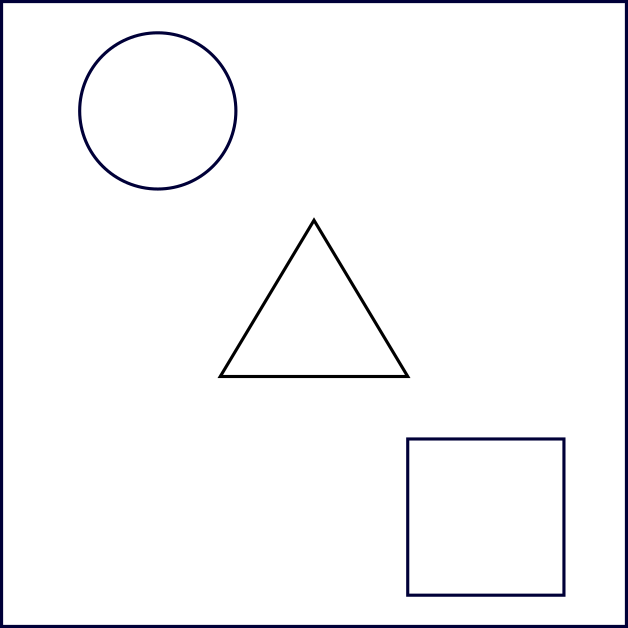
\includegraphics[width=40truemm]{fig-sample.png}
 \caption{\small{図の挿入例.}}
 \label{fig:sample}
\end{figure}

figure 環境中での label の位置は,caption よりも後に記述しなければならない.
この記述の順番を間違えると,
キャプション中と本文中で図番号がずれてしまうので注意すること.

なお,LaTeX での図用ファイルフォーマットは伝統的に EPS 形式が用いられてきたが,
現在の LaTeX では PNG,JPEG 形式といった主要画像フォーマットや PDF 形式のデータも
取り込むことが可能であり,適宜利用してもらって構わない.

表についても同様に,label を付加し,本文から label を用いて参照する.
一例として,以下の表 \ref{tab:sample} をご参照いただきたい.
表の label も図の場合と同様に,caption や表よりも後に記述すること.

\begin{table}[H]
 \caption{\small{表の挿入例.}}
 \centering
 \begin{tabular}{|c|c|c|c|}
	\hline
		& 数学	& 英語	& 国語	\\ \hline
	太郎	& 68	& 91	& 34	\\
	次郎	& 53	& 12	& 97	\\ \hline
 \end{tabular}
 \label{tab:sample}
\end{table}

本サンプルでは,図表の出現が tex ファイルの記述箇所と同一となるように,
figure 環境や table 環境のオプションに「H」を用いているが,
このオプションは適宜変更しても構わない.

また,図表を一段組で大きく描画したい場合は,
figure 環境や table 環境の末尾にアスタリスクをつけた
「\verb+\begin{figure*} 〜 \end{figure*}+」や
「\verb+\begin{table*} 〜 \end{table*}+」を用いる.
図 \ref{fig:sample-big} でその例を示す.

\begin{figure*}[ht]
 \centering
 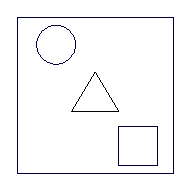
\includegraphics[width=60truemm]{fig-sample.eps}
 \caption{\small{一段組での図の挿入例.}}
 \label{fig:sample-big}
\end{figure*}

\subsection{数式}
数式のインラインモードは \(x^2 + y^2 \leq 1\) のように表示させることができる.
インラインモードで「\verb+$...$+」を使うやり方は,
近年の LaTeX ではあまり推奨されていないが,その利用は妨げない.

ディスプレイ数式モードを利用する際に推奨するのは equation 環境である.
\begin{equation}
	\bA_p = \frac{\bA\cdot\bB}{|\bB|^2}\bB .
	\label{eq:samp1}
\end{equation}
数式の参照は「\verb+\ref+」ではなく「\verb+\eqref+」を用いる.
上記の数式を参照すると「式\eqref{eq:samp1}」となる.
このように,\verb+\eqref+ を用いた場合は数式中と同じ様式の括弧がつく.

また,複数行にわたる数式を表示したい場合は align 環境を用いることを推奨する.
以下の式\eqref{eq:samp2}にその例を示す.

\begin{align}
	& \begin{bmatrix}
	a_{11} & a_{12} & \cdots & a_{1n} \\
	a_{21} & a_{22} & \cdots & a_{2n} \\
	\vdots & \vdots & \ddots & \vdots \\
	a_{m1} & a_{m2} & \cdots & a_{mn} \\
	\end{bmatrix}
	\otimes
	\begin{bmatrix}
	b_{11} & b_{12} & \cdots & b_{1n} \\
	b_{21} & b_{22} & \cdots & b_{2n} \\
	\vdots & \vdots & \ddots & \vdots \\
	b_{m1} & b_{m2} & \cdots & b_{mn} \\
	\end{bmatrix} \notag \\
	& \qquad \qquad = \sum_{i}^{m}\sum_{j}^{n}a_{ij}b_{ij} .
	\label{eq:samp2}
\end{align}

eqnarray 環境は,最近の LaTeX では幾つかのパッケージと同時に利用すると
問題が発生することがあるため,利用は推奨しない.

\subsection{参考文献}
参考文献は本文の後に全部まとめて列挙する.
すべての参考文献は本文中で引用する.
すべての参考文献には通し番号をつけるか,
固有の番号(例えば「\verb+[Ito04]+」など)をつけること.

本稿の末尾に,英語論文と日本語論文の参考文献の一例 \cite{Ito04}\cite{Abe10} を示す.
原則として,著者名,タイトル,掲載誌,(論文の場合には巻と号),
ページ数,発行年を記載すること.
書籍の場合には,書籍を特定する情報(出版社,ISBNなど)もできる限り記載すること\cite{Ito18}.
ウェブサイト\cite{ArtScience}を引用する場合には,参照日時も併記すること.
なお,本文中・参考文献中のいずれであっても,URLの表記は url パッケージを使用し,
「\verb+\url{https://....}+」コマンドを用いることを推奨する.

本ファイルは BibTeX を利用することを想定したサンプルとなっているが,
BibTeX を利用せずに参考文献リストを記述する場合は,
「BibTeXを利用しない場合」と記されている箇所のコメントアウトされている部分を
参照のこと.

\section{まとめ}

本稿では,NICOGRAPH をはじめとする芸術科学会学術会議投稿用の LaTeX 版サンプルを提供した.
本サンプルに不具合が発生した場合には,
芸術科学会にご一報をいただけると非常に幸いである.

%%%%%%%%%%%%%%%%%%%%%%%%%%%%%%%%%%%%%%%%%%%%%%%%%%%%%%%%%%%%%%%%%%%%%%%%%%%%%%
%%% 参考文献

%% BibTeX を利用する場合.(利用しない場合は以下の2行をコメントアウト)

\bibliography{bibtex_samp} % BibTeX ファイル (.bib) を記述
\bibliographystyle{junsrt} % 番号を掲載順にソートする.

%% BibTeX を利用しない場合
%
%\begin{thebibliography}{99}
%
% \bibitem{Ito04}
% T. Itoh, Y. Yamaguchi, Y. Ikehata and Y. Kajinaga.
% Hierarchical Data Visualization Using a Fast Rectangle-Packing Algorithm,
% IEEE Transactions on Visualization and Computer Graphics,
% Vol. 10, No. 3, pp. 302-313, 2004.
%
% \bibitem{Abe10}
% 阿部雅樹,渡辺大地.
% エネルギー波表現のリアルタイムレンダリング.
% 芸術科学会論文誌,Vol. 9,No. 3,pp.93--101,2010.
%
% \bibitem{Ito18}
% 伊藤貴之.
% 意思決定を助ける 情報可視化技術.
% コロナ社,2018.
% ISBN: 978-4339028836.
%
% \bibitem{ArtScience}
% 芸術科学会,芸術科学会論文誌,\url{https://art-science.org/journal/}.参照: 2019-1-1.
%
%\end{thebibliography}

\end{document}
